% FALTA el grafico access.eps
\graphicspath{ {img/SPEC_MAN/} }

\chapter[Uncertainty-Aware Opportunistic Spectrum Access in Coexistence-Friendly Systems][Uncertainty-Aware OSA in Coexistence-Friendly Systems]{Uncertainty-Aware Opportunistic Spectrum Access in Coexistence-Friendly Systems}\label{SPEC_MAN_chap}

\section{Introduction}\label{SPEC_MAN_sec_intro}
In our work on PU bandwidth reservation, described in the previous chapter, we have shown that the benefits of reduced PU-SU collisions outweigh the negative consequences of a more limited selection of channels available to the PUs. 
In this chapter we develop an OSA mechanism further exploiting that finding. 
We also continue improving MAC protocols for SUs with hardware-constrained cognitive radios, a sub-objective we began to pursue in chapter \ref{BD_chap}. More specifically, we address an issue that has not received much attention in multi-channel OSA protocols: the increase in the uncertainty of channel occupancies with the elapsed time from the observations.  
\subsection{Motivation}
Let us consider a system where a hardware-constrained cognitive transmitter intends to transfer some data to a cognitive receiver using one or several narrowband channels within certain licensed spectrum band (\textit{multi-channel} access). 
Specifically, the hardware constraints imply that: (1) fine sensing can only be conducted within a small portion of spectrum (sensing constraint) at a time; (2) the spectrum used by an SU has a limited bandwidth (transmission constraint) and (3) SUs are equipped with a single cognitive radio which cannot sense and transmit simultaneously.
After a contention phase, these SUs (cognitive pair) start to scan the spectrum in consecutive periods (scanning slots) in order to detect which channels are free of PU activity and thus available for transmission. 
During each scanning slot, the cognitive pair (CP) senses only one channel and the SUs exchange messages informing each other about the observation outcome.
Therefore, each scanning slot introduces a time overhead that needs to be considered in the OSA protocol design.
After each scanning slot, the cognitive pair has to decide whether to continue scanning or to transmit (and how many channels to transmit in).

Optimizing this process is challenging because of the trade-offs involved. 
On the one hand, sensing more channels allows the SU to find more available channels to transmit in, potentially achieving higher throughput.
But on the other hand, the scanning time overhead increases as more channels are sensed, which is contrary to the throughput goal.
In addition, \textit{using many scanning slots implies more uncertainty about the information obtained in earlier slots}: the channel occupancy of earlier sensed channels may have changed before the SU transmission (\textit{scanning delay}).
In a real system, where sensing results are not fully reliable, this uncertainty is even higher.
To the best of our knowledge, this last aspect has never been included in a sequential sensing mechanism with multichannel access, and is the first key issue addressed in this chapter. 

The second key issue is \textit{to evaluate the impact of the channel allocation scheme for PUs on OSA performance}.
If each channel is randomly occupied by a PU, both the collision probability and the post-scanning uncertainty variation over time is the same for every channel.
However, the licensed operator could allocate its channels to the PUs with a different pattern, more friendly to the coexistence with OSA nodes.
Specifically, we show that a simple sequential channel assignment for PUs reduces collisions with SUs. In addition, if the licensed network has the ability to aggregate channels with ongoing PU sessions into a compacted spectrum block (\textit{spectrum merging}), the reduction is even greater.
It is easy to see that SUs' throughput will be dramatically improved. 
On the other hand, for primary systems that can dynamically change the channels assigned to ongoing PU transmissions, using these policies reduces the ability of the base station to exploit the channels with best instantaneous propagation conditions. In those cases, the negative impact in PUs' throughput is compensated by the effect of the reduced collisions, under certain traffic intensities, as shown in the previous chapter and is also highlighted in \cite{ref:ElSawy2013}. For other scenarios, the reduction in PUs' throughput due to spectrum merging is minimal.

Obviously, this OSA framework requires the SU nodes to have a previous knowledge of PU traffic descriptors. 
This is a typical requirement for OSA protocols, and multiple previous works offer solutions to this problem.  
However, traffic estimations are generally imperfect.
Therefore, we also evaluate the impact of the difference between estimated and real PU traffic parameters. 
Our findings show that this difference has a surprisingly low impact on PU performance.

\subsection{Related Work}\label{SPEC_MAN_sec_related_work}
MAC designs for hardware-constrained radios were introduced in \cite{ref:Jia2008_HC}. However its authors focused only on optimizing SU's throughput and did not provide a method to compute the actual overlapping time which is one of the objectives of our model. In addition, it uses a worst case approach, setting a fixed duration of $T$ seconds for SU transmissions, where $T$ is the maximum overlap time with SU activity that a PU receiver could tolerate.

Several works consider multichannel access with sensing constraint \cite{ref:Kim2008,ref:Gabran2011,ref:Cheng2011}. The proposal in \cite{ref:Kim2008} optimizes the discovery of spectrum opportunities. In contrast to our model, the system in \cite{ref:Kim2008} is assumed to be collision-free. In \cite{ref:Gabran2011}, the focus is on optimizing the sensing phase considering, among other aspects, the trade-off between its duration (and reliability) and collision probability. As we will explain later, our model incorporates similar considerations, but in the design of access policies that include not only the sensing phase but also the number of channels to transmit in. Finally, the approach in \cite{ref:Cheng2011} is perhaps the closest to ours, although there are two significant differences: first, \cite{ref:Cheng2011} aimed to optimize SU's throughput without quantifying the effect on PU's performance. Second, our formulation incorporates the increase in the uncertainty of past channel observations over time, which is crucial for evaluating the effect of PU channel allocation schemes.

Other works consider the uncertainty increase over time, but only across different sensing episodes, not during the ongoing one. Those works propose models with either single channel sensing and immediate transmission \cite{ref:Zhao2008,ref:Filippi2011}, or with a fixed \textit{a priori} set of channels to sense \cite{ref:Zhao2007_dec,ref:Berthold2008,ref:Lunden2011}. In contrast, we aim at an optimal multichannel access strategy, which implies that the number of channels scanned on any sensing episode must depend on the sequence of observations received during this episode.
%Other works also include such uncertainty increase with time, but only across different sensing episodes, not as part of a sequential sensing decision problem and posterior multichannel transmission. Those works propose models with either single channel sensing and immediate transmission \cite{ref:Zhao2008,ref:Filippi2011} or with a fixed \textit{a priori} set of channels to sense \cite{ref:Zhao2007_dec,ref:Berthold2008,ref:Lunden2011}. As opposed to ours, those designs cannot adapt their decision to the observations obtained during the ongoing sensing period.   

%The PU bandwidth reservation issue was addressed in \cite{ref:Alcaraz2013}, where we showed that the benefits of reduced PU-SU collisions outweigh the negative consequences of a more limited selection of channels available to the PUs. 
%%This allows us to focus on avoiding collisions in this work and therefore, to safely simplify the PU's QoS metric to the overlapping time, as opposed to more complex but preferred metrics \cite{ref:Sun2012} such as�interference level at PU receivers or PN Shannon capacity.
%In works where PU's QoS is addressed, it is usually characterized by collision probability: \cite{ref:Gabran2011,ref:Jung2012,ref:Zhao2007_dec,ref:Huang2009,ref:Jung2012}. 
%Fewer works \cite{ref:Huang2008} consider overlapping time which,
%as stated in \cite{ref:Huang2009}, is closely related to packet collision probability. 
%%It is a common assumption to consider any overlapping time equivalent to a packet collision. 
%%However, a more precise conversion involves many features such as capture effect, bit interleaving and forward error control techniques.
%We use the overlapping time to characterize the PU's QoS, which is more conservative than other metrics such as signal to interference ratio, or packet error probability. Note that not all the overlapping time results in harmful interference or packet reception errors at the PU receivers, therefore using this metric enables a worst-case approach.
%%Therefore, because of its greater generality, we adopt overlapping time as the PU's QoS parameter.


The previous chapter and this work are in line with the recent increase of interest in non-transparent access of SUs to PUs' spectrum \cite{ref:Mao2010,ref:Kay_Tang2009}. This trend is in contrast to the traditional approach maintained since the origin of cognitive radio \cite{ref:Mitola2000}, specially under the spectrum interweave OSA model \cite{ref:Zhao2007_dec}. 
Such change of paradigm is probably motivated by the application of OSA techniques to heterogeneous cellular networks (HetNets). 
HetNets also imply overlay networks (small cells, often with cognitive abilities, over the macro-cell network), but a substantial difference with classical interweave OSA: that all the HetNet users are PUs and thus, QoS must be guaranteed for both the macro and the small cell users. 
Because of this, in an HetNet scenario, it is intuitively convenient for the operator to be coexistence-friendly with its associated small-cells, even though they implement cognitive abilities. 
While some works \cite{ref:ElSawy2013,ref:Lima2012} have studied channel assignment policies for HetNets, the design of optimal multichannel OSA strategies in coexistence-friendly environments is still an open issue. 
%In \cite{ref:ElSawy2013}, H. ElSawy and E. Hossain study a random and a sequential channel assignment strategy for macro-cell users in a two-tier network.


%Apart from the different context, other important differences with our work are that: their cell deployment model is based on stochastic geometry, and inter-cell interferences must be taken into account; we additionally propose the novel spectrum merging strategy; they do not model the users' access strategies; and they assume perfect spectrum sensing.
%Although \cite{ref:Lima2012} also considers resource allocation strategies, the sensing capabilities.  

%%In the framework of spectrum trading (which is also non-transparent to the PN), works such as \cite{ref:Wu2012} and \cite{ref:Biglieri2013} feature bandwidth reservation for future leasing. Nevertheless, spectrum trading requires the implementation of new protocols to support the required PU-SU signaling and makes the spectrum sensing no longer needed. It is therefore essentially different to the opportunistic access framework of our proposal. 

%Also in the spectrum trading context, \cite{ref:Maille2009} features a competitive duopoly where the operators have license to transmit in a fixed spectrum band and can access a shared unlicensed one under congestion. This can be seen as a sort of sequential allocation. However, the objective of the paper is significantly different to ours. It addresses the equilibrium of the operators' pricing strategies and its effect on their profits and their suscribers' welfare. 

%We are also interested in evaluating the effect of PU spectrum usage on the overall performance, therefore we devote special attention to aspects related to PU activity characterization.
%The first one is the timescale associated to each type of users. When SUs are assumed to operate in a much faster timescale than PUs, the spectral environment is treated as static. On the contrary, we consider that PU and SU activity periods have similar timescales, similarly to the works previously cited.
%The second aspect is the time structure of PU communications, that can be slotted as in \cite{ref:Gabran2011}, \cite{ref:Cheng2011}, \cite{ref:Zhao2007_dec}, \cite{ref:Huang2009} and \cite{ref:Park2011} where PUs are assumed to arrive and depart at discrete times that are multiples of the slot duration.

%We adopt unslotted PU communications as in \cite{ref:Kim2008}, \cite{ref:Jung2012} and \cite{ref:Huang2008}, despite its higher analytic complexity because it is more accurate for computing overlapping time, and does not require the assumption of PU and SU synchronization.
%%The third aspect is PU traffic characterization and scope. For traffic modeling we use the exponential distribution, historically used to characterize call durations in communication systems, and considered also suitable to model PU channel holding times as done in \cite{ref:Kim2008}, \cite{ref:Huang2008} and \cite{ref:Tang2009}. 
%Regarding the scope of PU activity model, most works restrict it only to the channel where the SU is operating (\textit{e.g.} \cite{ref:Kim2008}, \cite{ref:Park2011}) while fewer ones (\cite{ref:Gabran2011} ,\cite{ref:Zhao2007_dec}) extend the model to all the channels in the spectrum band. However, every mentioned work essentially assumes that each channel can be randomly and independently occupied by a PU. In contrast, our research objectives require modeling all the channels but considering different occupation patterns. 


\subsection{Our Contribution}
%The goal of this work is to find and characterize OSA policies for SUs with the hardware limitations described previously and to evaluate the impact of PU channel allocation mechanisms.
This chapter comprises the following main contributions: 
\begin{enumerate}
\item We address an issue that has been largely ignored in the design of multi-channel OSA protocols for hardware constrained radios: considering the effect of the scanning delay in the uncertainty of the information available at the SUs. Finding an optimal OSA strategy implies solving a Partially Observable Markov Decision Process (POMDP) with finite horizon. This is a challenging task because of the inherent complexity of POMDPs, which is increased by the inclusion of delay-dependent uncertainty.
%We develop an optimal SU access strategy that considers the effect of scanning delay in the uncertainty of the information available at the SUs. This effect has been largely ignored in the design of OSA protocols for hardware limited radios. 
\item The OSA scheme is designed and evaluated for different levels of \textit{coexistence friendliness} at the spectrum owner, reflected on its spectrum management policies. Specifically: random allocation, sequential allocation and sequential allocation with spectrum merging. We also show how the selected spectrum management policy relates to the delay effects considered in the OSA design.
\end{enumerate}

%Existing research had addressed the trade-off imposed by the scanning delay: scanning more channels allows the SU to transmit in more channels simultaneously but also increases the delay overhead.
%Part of our contribution is to include another key element into the model: the effect of the scanning delay on the reliability of the observations, which is crucial when considering PU activity in all the spectrum band.
%the effect of the scanning delay on the reliability of the observations. 
%In addition, our contribution comprises the following items:
%\begin{itemize}
	%\item Formulating the CP decision problem as a finite horizon Markov decision process (MDP) with imperfect state estimation, handling the partial and unreliable knowledge that the SU has about the spectrum occupation.&	\item Characterizing QoS of PUs by means of the activity overlap with SU communications (\textit{overlapping time}) and studying the trade-off with SU throughput.
	%\item Analyzing computational and memory overhead of the proposed OSA framework.
	%\item Quantifying the influence of PU channel management strategies on global performance.
	%\item Evaluating the robustness of OSA policies to PU traffic estimation inaccuracies.
	%\item Extending the model to imperfect spectrum sensing.
%\end{itemize}

%Designing the optimal OSA protocol implies solving a Partially Observable Markov Decision Process (POMDP) with finite horizon. This is a challenging task because of the inherent complexity of POMDPs, which is increased by adding the effect of the scanning delay on the reliability of past observations. 

%In the existing literature this delay had been associated to one relevant trade-off: more scanning time allows the SU to discover more available bandwidth but also increases the delay overhead. We refine this trade-off by adding the effect of the delay on the information uncertainty.

%Because the MDP problem comprises two opposite objectives, SU throughput and overlapping time, solving the MDP implies finding Pareto-optimal policies. A policy is Pareto-optimal if one of the objectives can only be improved by worsening the other.
%We make use of Pareto fronts to compare policies and spectrum management schemes as well as to quantify the trade-off between QoS parameters.
%Note that the computational overhead of solving the MDP may be unfeasible for an SU. Nevertheless it is not required in practice, since the optimal policy can be computed off-line and simply stored in every SU. 

\section{System Description}\label{SPEC_MAN_sec_system}
\subsection{Licensed Network}
The system under study consists of two overlay wireless networks. The licensed one operates with centralized access coordinated by an access node (AN). The spectrum used by this network comprises $N$ adjacent narrowband channels. %Upon a PU arrival, the AN assigns one of these channels, if available, to the incoming PU.
Upon each PU arrival, the AN assigns an available channel to the incoming PU.
SU activity is not detected by either the PUs or the AN, therefore a PU may occupy a channel with an ongoing SU transmission.
Similarly to many related works (\textit{e.g.} \cite{ref:Zhao2007_dec}, \cite{ref:Kim2008}, \cite{ref:Tang2009}), PU traffic is assumed to follow a Poisson model: PU inter-arrival time characterized by an exponential random variable with rate $\lambda$ and channel holding time described by an exponential random variable with rate $\mu$.

The criteria for PU channel allocation depend on the system, \textit{e.g.} the AN may assign them according to channel quality measurements reported by the PUs. So far, in OSA research it has been usually assumed that channels are occupied by PUs according to independent identically distributed (i.i.d.) processes. In that scheme, that we refer to as \textit{random allocation}, every channel can be assigned to an incoming PU with the same probability.
However, when the same spectrum band is accessed by opportunistic nodes, random allocation is not optimal in terms of collision probability. In this work we investigate the benefits of using different spectrum management strategies for allocating channels to PUs. Therefore, we consider two additional schemes:
% Therefore, in addition to the random allocation described previously, we consider two other schemes:
\begin{enumerate}
	\item \textit{Sequential allocation}: Considering the $N$ channels numbered from $1$ to $N$, each incoming PU is always assigned the highest numbered available channel.
	\item \textit{Sequential allocation with spectrum aggregation}: channels are assigned to PUs sequentially, es explained before, but when one PU releases its channel, all the spectrum currently in use by ongoing PU communications is rearranged so that all the active PUs occupy the adjacent channels with the highest numbers (merged spectrum).  
\end{enumerate}
Fig. \ref{fig:allocation} illustrates the arrival and departures of PUs under these allocation schemes.
\begin{figure}[ht]
\centering
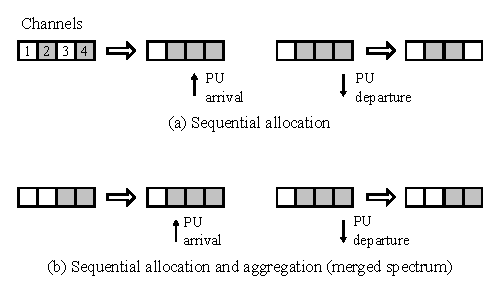
\includegraphics[scale=1]{allocation.eps}
\caption[]{Channel allocation schemes for PUs.}\label{fig:allocation}
\end{figure}
Many wireless access systems, \textit{e.g.} OFDMA-based systems, allow both sequential allocation of channels (subcarriers) and channel rearrangement for ongoing communications.
However, in some cases, sequential allocation may imply assigning channels whose propagation conditions are not optimal for the incoming PUs.
For those cases, we assume that the AN uses the bandwidth reservation scheme of the previous chapter, which would be equivalent to spectrum merging. In that chapter it was concluded that the benefits of easing secondary access overcome its drawbacks when the primary traffic intensity is below certain threshold. Therefore, the use of a coexistence-friendly spectrum management scheme implies the implicit assumption that the PU traffic intensity is below that threshold, which is reasonable since OSA is conceived to increase the efficiency of underused spectrum of, e.g. legacy networks.

\subsection{Secondary Network}
The unlicensed or secondary network operates in a decentralized, ad-hoc fashion. 
Communication is always performed between pairs of SUs (\textit{cognitive pairs}) consisting of one sender and one receiver.
Every SU is assumed to be under the coverage area of the same licensed access node, thus the SU's objective is to transmit data using one or several of the $N$ licensed channels causing the less possible interference to PU communications.
Secondary nodes are constrained to some hardware limitations:
(1) Each SU is equipped with a single radio that can either transmit or receive, but not at the same time.
(2) When sensing the spectrum to detect PU activity, an SU can only sense one of the $N$ channels.
(3) Once a cognitive pair decides to start a transmission, it can use up to $M$ noncontiguous channels simultaneously.
%Once a cognitive pair decides to start a transmission, the sender SU can use several channels simultaneously. There is, however a limit on the width of the spectrum aggregated in a SU transmission. This limit is set to $M$ channels.

%The SUs implement the MAC protocol (HC-MAC) described in \cite{ref:Jia2008_HC} with a different sensing and accessing decision policy. 
%HC-MAC comprises three phases that we briefly summarize here:
%\begin{enumerate}
%	\item \textit{Contention}: When an SU sender wants to establish a connection it listens the dedicated control channel to assess ongoing SU activity. If no SU is reporting activity, the sender node transmits a contention message (C-RTS) to the target node on the control channel. The receiver node then replies with a C-CTS. This procedure allows the cognitive pair to reserve time for the following sensing and transmission phases as well as to synchronize both nodes.
%	\item \textit{Sensing}: After winning the contention, both the sender and the receiver SUs start to scan the spectrum in consecutive, synchronized stages (\textit{sensing slots}). During a sensing slot both nodes listen to the same single channel and share the sensing results by exchanging S-RTS/S-CTS messages. After each sensing slot the cognitive pair decides whether to finish or to continue the sensing phase. 
%	\item \textit{Transmission}: Once the cognitive pair finishes the sensing phase the sender node begins to use a set of available channels to transmit data packets during a period of $T$ units of time. After finishing the transmission, both nodes exchange T-RTS/T-CTS packets notifying neighboring nodes the release of the reserved resources. Upon receiving this notification, neighboring nodes listening the control channel will contend after a random backoff period.
%\end{enumerate}
The SUs implement the MAC protocol described in \cite{ref:Jia2008_HC} (HC-MAC) with a different sensing and accessing decision policy. Summarizing, HC-MAC comprises three consecutive phases: \textit{contention}, \textit{sensing} and \textit{transmission}. 
The contention procedure allows a pair of SUs (sender and receiver) to reserve the use of the spectrum in a certain area avoiding collisions with other SU transmissions. 
After winning a contention, the cognitive pair starts to sense the spectrum in fixed-duration sensing slots.
%during which both the sender and the receiver sense the same channel and exchange the sensing result. Let $\tau$ denote the duration of a sensing slot. 
During the $\tau$ seconds of each slot both the sender and the receiver sense the same channel and exchange the sensing result.
% upon which a decision is made whether to sense the next channel or to transmit using one or more of the available channels detected. 
At the end of every slot, a decision is made whether to sense the next channel or to transmit using one or more of the available channels detected. 
Because of the information exchange, the cognitive pair acts as a single entity when making the transmission decision provided that both nodes operate under the same policy.
%RTS/CTS exchange procedures in each phase prevent collisions among SU transmissions.
Similarly to \cite{ref:Jia2008_HC} and \cite{ref:Park2011}, in case of overlapping with PU activity, the SU transmission is considered to be successful, \textit{i.e.,} it is assmmed that the received power at the SU receiver from the corresponding SU transmitter is much higher than the interference from PUs. Nevertheless, since the model also estimates the expected overlapping time at each state, it could be readily extended to the case in which the SU transmissions can be harmed by PU interference.

The OSA policy considered in this work differs from the one in HC-MAC in its decision space and its computation procedure.
We use an extended decision space such that instead of using the total number of available channels, the sender may use any smaller number, including quitting the sensing process without transmitting. 
%$0$ channels (quitting decision). 
%extended decision space, so that in the transmission phase the set of used channels may range between $0$ and the total number of available channels. 
The differences in policy computation result from a more general formulation incorporating aforementioned aspects, namely: observation uncertainty due to imperfect sensing and delay overhead; modeling PU activity on the whole spectrum band with diverse channel allocation strategies; and PU's QoS characterization in terms of overlapping time.
Fig. \ref{fig:access} depicts a simplified example of SU access incurring in an overlapping event. 
%Reducing the expected duration of the overlapping periods is one of the goals of OSA policy design.
\begin{figure}
\centering
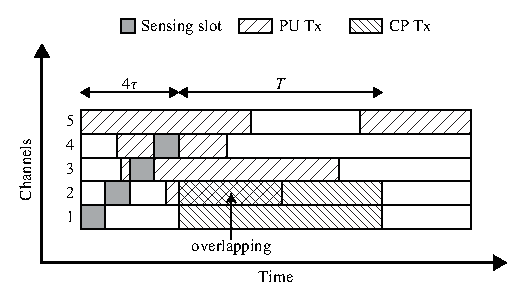
\includegraphics[scale=1]{access.eps}
\caption[]{OSA example. After sensing channels 1 to 4, the CP decides to transmit in channels 1 and 2, resulting in an overlapping event on channel 2.}\label{fig:access}
\end{figure}
%EXPLICAR QUE ANTE UN OVERLAP SE ASUME QUE EL SU RECIBE LOS PAQUETES.
%SE PUEDE TRANSMITIR EN HASTA M NONCONTIGUOUS BANDS
%SOLO SE PUEDE TRANSMITIR O SENSORIZAR EN UN SLOT
%ACLARAR QUE EL SENSING SLOT TAMBI�N INCLUYE EL CHANNEL SWITCHING TIME

%The differences in policy design and computation respect HC-MAC are
%\begin{enumerate}
%	\item \textit{Modeling PU activity} over the whole spectrum band incorporating different channel allocation strategies. We use the more general continuous time approach instead of slotted time.
%	%\item \textit{PU QoS} characterized by the time of overlapped activity between PUs and SUs on the same channels.
%	\item \textit{PU QoS} characterized by the amount of time that each channel contains simultaneous activity of PUs and SUs.   
%	\item \textit{Extended decision space}, so that in the transmission phase the set of used channels may range between $0$ and the total number of available channels.
%\end{enumerate}

%Describir la red en la que se desarrolla el sistema y el protocolo de acceso. 
%Conceptos a destacar:
%spectrum aggregation. Multichannel transmission. Hardware constraints. Sensing time. Transmission time. 
%aspecto novedoso: channel allocation patterns.
%motivations: maximizar el throughput. disminuir el tiempo medio en el que se solapan transmisiones de usuarios primarios y secundarios.

%La propuesta de reorganizar la asignaci�n de canales a los PU no colisiona con las decisiones de scheduling ya que, por definici�n OSA es factible solo en situaciones de bajo uso del espectro por parte de los usuarios primarios, que es cuando aparecen spectrum holes, y en cuyo caso el scheduling is not an issue.

%En nuestro sistema se propone emplear tiempo de colisi�n al considerarlo m�s general que probabilidad de colisi�n ya que en muchos casos, las t�cnicas FEC permiten recuperar el mensaje cuando el n�mero de s�mbolos erroneos es peque�o. Por tanto, a mayor tiempo de colisi�n mayor es el n�mero de s�mbolos err�neos. Adem�s, el el n�mero de bits por s�mbolo puede variar de un PU a otro, por lo que la probabilidad de error de bit tambi�n varia. 
%En cualquier caso, si se minimiza el tiempo total esperado en el que se solapan las actividades de los PU y los SU se garantiza la calidad de servicio de los PU.
\section{POMDP Formulation}\label{sec:Models}
%Diferenciar entre el modelo de red y el modelo del cognitive user. Procesos Y(t): spectrum state y \vec{X}_{k}. 
%Porceso de llegada y salidas de los usuarios primarios a la red tipo Poisson.
%Definir tasa de llegadas $\lambda$ y tasa de salidas $s$.

%our model possesses the same limitations as those in \cite{ref:compartivaMAC}.
%due to the significant involvement of the delay analysis, the model is limited to throughput assessment only. In addition, this work is limited to a single collision domain, and effects such as hidden/exposed terminals are not modeled.

In this section we formulate the opportunistic access problem as a POMDP with finite horizon and obtain an equivalent MDP by means of the \textit{state augmentation} approach. 
The formulation in this section uses a generic objective, and therefore it is applicable to any optimization criterion, e.g. increasing SU throughput, capacity, etc. Section \ref{sec:Policies} describes the computation of a specific cost function balancing SU throughput and overlapping time.
%We follow a top-down approach to describe the model. 
%We use in this section in order to provide a general understanding of the POMDP framework, and becomes more specific in Section \ref{sec:Policies}.

\subsection{The Spectrum Process}
Considering only PU activity, each of the $N$ channels can be in two states: $1$, when the channel is assigned to one PU, and $0$ when the channel is unassigned.
Let $Y(t)$ denote the aggregate state of the $N$ channels at time $t$. $Y(t)$ is a continuous-time Markov chain (CTMC) that we refer to as the \textit{spectrum process}. Each channel allocation scheme results in a different stochastic behavior for $Y(t)$.
The set of (countable) values that $Y(t)$ can take, is denoted by $\mathcal{S}$. Let $i$, $j$ $\in \mathcal{S}$ be two states of $Y(t)$ and let $\left(i\right)_{2}$ denote the binary representation of $i$ as an $N$-tuple, \textit{i.e.} $\left(i\right)_{2} = \left(i_{1},\ldots,i_{N}\right)$, where $i_{k} = 1$ if the $k$-th channel is occupied by a primary user and $i_{k} = 0$ otherwise. We will also refer to $i_k$ as the state of channel $k$. The complementary of $\left(i\right)_{2}$ is denoted by $\overline{\left(i\right)_{2}}$.
The 1-norm of $\left(i\right)_{2}$ is defined as
\begin{equation}\label{1Norm}
\left\|\left(i\right)_{2}\right\|_{1}=\displaystyle\sum_{k=1}^{N}\left|i_{k}\right|
\end{equation}
Note that previous expression provides the number of occupied channels in the system while $\left\|\overline{\left(i\right)_{2}}\right\|_{1}$ yields the number of free channels.

Table \ref{Table_markovian_models} summarizes, for each channel allocation scheme, the set $\mathcal{S}$, and the elements $q_{ij}$ of infinitesimal generator, $\mat{Q}$, of $Y(t)$.
%We summarize $\mathcal{S}$, and the components of the infinitesimal generator $\mat{Q}$ characterizing $Y(t)$, $q_{ij}$, for each scheme in table \ref{Table_markovian_models}.

\begin{table*}
\small
\begin{tabular}{lcC{8cm}} 
\hline
& $\mathcal{S}$ & $q_{ij}$\\\hline
Random & 
$\left\{0,1,\ldots,2^N\right\}$ &
\parbox{7cm}{\begin{equation*}\label{Qrandom}
    \begin{cases}
    \frac{\lambda}{\left\|\overline{\left(i\right)_{2}}\right\|_{1}}, & \mbox{if} \quad \sum_{n=1}^{N}\left(j_{n}-i_{n}\right) = 1\\
  
    \mu, & \mbox{if} \quad \sum_{n=1}^{N}\left(i_{n}-j_{n}\right) = 1 \\

    -\lambda - \left\|\left(i\right)_{2}\right\|_{1}\mu, & \mbox{if} \quad i = j\\
    
    0, & \mbox{otherwise}\\
    \end{cases}
\end{equation*}}\\
Sequential &
$\left\{0,1,\ldots,2^N\right\}$ &
\parbox{7cm}{\begin{equation*}\label{Qordered}
    \begin{cases}
    \lambda, & \mbox{if} \quad j = i + 1\\
  
    \mu, & \mbox{if} \quad \sum_{n=1}^{N}\left(i_{n}-j_{n}\right) = 1 \\

    -\lambda - \left\|\left(i\right)_{2}\right\|_{1}\mu, & \mbox{if} \quad i = j\\
    
    0, & \mbox{otherwise}\\
 \end{cases}
\end{equation*}}\\
Merged & 
$\left\{0,1,\ldots,N\right\}$ &
\parbox{5cm}{\begin{equation*}\label{Qcompacted}
    \begin{cases}
    \lambda, & \mbox{if} \quad j = i + 1\\
  
    i\mu, & \mbox{if} \quad j = i - 1\\

    -\lambda - i\mu, & \mbox{if} \quad i = j\\
    
    0, & \mbox{otherwise}\\
 \end{cases}
\end{equation*}}\\\hline 
\end{tabular}
\centering
\caption{State space $\mathcal{S}$ and components of the infinitesimal generator $\mat{Q}$ characterizing $Y(t)$ for random channel allocation, sequential channel allocation, and sequential allocation with spectrum merging.}
\label{Table_markovian_models}
\end{table*}

%\subsection{POMDP Model of the Cognitive Pair}

%Let us briefly summarize the medium access strategy of the secondary users (SUs). This strategy is basically divided into three consecutive periods: \textit{contention}, \textit{sensing} and \textit{transmission}. After winning a contention, a pair of secondary users (sender and receiver) starts to sense the spectrum in fixed-duration sensing slots, during which both the sender and the receiver sense the same channel and exchange the sensing result. Let $\tau$ denote the length of a sensing slot. After each slot a decision is made whether to sense the next channel or to transmit using one or more of the available channels detected. Because of the information exchange at each sensing slot, the cognitive pair acts as a single entity when making the transmission decision provided that both nodes operate with the same policy.

\begin{table}
\begin{tabular}{ll}\hline
\textbf{Notation} & \textbf{Definition}\\\hline
$N$& number of channels in the spectrum band\\
$M$& maximum usable channels by the CP\\
$k$& scanning slot (decision stage) \\
$\tau$& duration of a scanning slot \\
$T$& duration of a CP transmission\\
$R$& data rate of a single channel\\
$Y(t)$& state of the spectrum process at time $t$\\
$Y_{k}$& value of $Y(t)$ at the end of $k$-th scanning slot\\
$\mathcal{S}$& state space of $Y(t)$ (and $Y_{k}$)\\
$\mat{Q}$& infinitesimal generator of $Y(t)$ \\
$q_{ij}$& elements of $\mat{Q}$\\
$\lambda$& arrival rate for PU population\\
$\mu$& PU departure rate\\
$\mat{P}$ & transition probability matrix for $Y_{k}$ \\
$p_{ij}$ & elements of $\mat{P}$\\
$Z_{k}$ & sensing outcome on channel (and slot) $k$\\
%$\vec{X}_{k}$ & information vector at the CP\\
$X_{k}$ & state (information vector) of the CP system\\
$\mathcal{S}(k,s_{k})$ & states in $\mathcal{S}$ such that channel $k$ is in state $s_k$\\
$\mathcal{X}_{k}$ & state space of the information vector\\
%$\mathcal{X}^{*}_{k}$ & state space of the CP system\\
$p_{\bar{p}}$ & probability of false positive detection\\
$p_{\bar{n}}$ & probability of false negative detection\\
$u_{k}$ & scanning decision at stage $k$\\
$m_{k}$ & selected channels at stage $k$\\
$d_{k}=(u_{k},m_{k})$& CP decision at stage $k$\\
%$\mathcal{U}_{k}$ & control space for $u_{k}$\\
%$\mathcal{M}_{k}(x_{k})$ & control space for $m_{k}$\\
$\mathcal{D}_{k}(x_{k})$ & control space for $d_{k}$\\
$\mu_{k}(x_{k})$ & function mapping CP states to decisions\\
$g_{k}\left(x_{k},d_{k}\right)$ & per-stage cost of the CP system\\
$\eta$ & admissible policy for the CP system\\
$J_{\eta}$ & cost function for policy $\eta$ \\
$J^{*}$ & optimal cost for the CP system\\
%$p_{k}\left(x_{k+1} | x_{k}, u_{k}\right)$ & transition probability of the CP system\\
$p_{k}\left(\ast|\ast\right)$ & transition probability of the CP system\\
%$P\left(\vec{X}_{k}=x_{k}|x_{k-1}\right)$ & transition probabilities for $\vec{X}_{k}$\\
$\vec{\pi}_{x_{k}}$ & \textit{a posteriori} estimation of $Y_{k}$ given $x_{k}$\\
$\hat{\vec{\pi}}_{x_{k}}$ & \textit{a priori} estimation of $Y_{k+1}$ given $x_{k}$\\
$b_{\text{max}}$ & maximum achievable throughput by the CP\\
$b_{k}(m_{k})$ & throughput attained with decision $m_{k}$\\
$c_{\text{max}}$ & maximum overlapping time\\
$c_{k}(x_{k},m_{k})$ & expected overlapping time given $x_{k}$ and $m_{k}$\\
$l_{i,x_{k}}(t)$ & expected time of $Y(t)$ in $i$ given $x_{k}$\\\hline
\end{tabular}
\centering
\caption{Summary of notation}
\label{Table1}
\end{table}

\subsection{Partial Observations and the Information Vector}
%Definir mejor z, Z, x, X y los espacios de estados en los que est�n definidos.
%As explained in previous subsection, the \textit{spectrum process} is a CTMC denoted by $Y(t)$. At time $t$, $Y(t)$ can be at any state $i \in \mathcal{S}$.
%We used $i_{n} \in {0,1}$ with $n \leq N$ to refer to the $n$-th element of the binary representation $\left(i\right)_{2}$ of state $i$, and denotes the state (idle or occupied) of the $n$-th channel.
The cognitive pair \textit{partially observes} $Y(t)$ in consecutive periods (scanning slots) of $\tau$ seconds.
%However, it only observes $Y(t)$ \textit{partially}.  
%During each scanning slot only one of the channels of the spectrum is observed.
%, \textit{i.e.} only one element of the binary representation $\left(i\right)_{2} = \left(i_{1},\ldots,i_{N}\right)$ is observed. 
%At the end of the $k$-th scanning slot an observation $z_{k}$ is obtained. 
In particular, during the $k$-th scanning slot, only the $k$-th channel of the spectrum is sensed.
At the end of the sensing slot, the CP obtains the sensing result $z_{k}$: $z_{k}=1$ if the $k$-th channel is estimated to be occupied, or $z_k=0$ otherwise.
Therefore, $z_k$ is a partial (and possibly unreliable) observation of $Y(t)$.
%At the end of this slot an observation $z_{k}$, the sensing result, is obtained.
%OSA decisions should be made according to these partial observations. 
Hence, we face a POMDP problem, which implies that decisions should be based on \textit{imperfect state information}.
Moreover, note that the observations $z_k$ obtained in consecutive scanning slots $k=1,2,\ldots$, correspond to samples of $Y(t)$ taken in different instants. Let us formalize these aspects and their implications.

%descripci�n del proceso Z_{n}
Let us define the \textit{observation process} $Z_{k}$ taking values from the observation space $\left\{0,1\right\}$. We assume that the channel activity detection depends on the values of the spectrum process at the end of each slot. Therefore we define the discrete-time Markov chain (DTMC)
\begin{equation}
Y_{k} = Y\left(k\tau\right), \quad \mbox{for }k = 1,\ldots,N.
\end{equation}
The observations are originated, in general as
\begin{equation}
Z_{k} = h_{k}\left(Y_{k}\right), \quad \mbox{for }k = 1,\ldots,N.
\end{equation}
%The observation $Z_{k}$ belongs to the observation space $\left\{0,1\right\}$. 
Assuming perfect detection and $Y_{k} = i$, with binary representation $\left(i\right)_{2} = \left(i_{1},\ldots,i_{N}\right)$, the function on the right hand side has the following form:
\begin{equation}
h_{k}\left(i\right) = i_{k}, \quad \mbox{for }k = 1,\ldots,N.
\end{equation}
In case the detection process is subject to errors such as false positive and false negative detections characterized by the probabilities $p_{\bar{p}}$ and $p_{\bar{n}}$ respectively, the function $h_{k}\left(i\right)$ provides random values in the observation space according to the following conditional distribution:
\begin{equation}
\begin{array}{lcl}
P\left(h_{k}\left(i\right)=1|i_{k}=1\right) & = & 1 - p_{\bar{n}}\\
P\left(h_{k}\left(i\right)=0|i_{k}=1\right) & = & p_{\bar{n}}\\
P\left(h_{k}\left(i\right)=1|i_{k}=0\right) & = & p_{\bar{p}}\\
P\left(h_{k}\left(i\right)=0|i_{k}=0\right) & = & 1 - p_{\bar{p}}
\end{array}
\end{equation}
for $k$ = $1,\ldots,N$.

The observation process $Z_{k}$ is a DTMC. To show this fact, let us define the set $\mathcal{S}(k,s_{k})$ containing the states in $S$ such that channel $k$ is in state $s_k$:
\begin{equation}\label{setS}
\mathcal{S}(k,s_{k}) = \left\{i \in \mathcal{S}|i_{k} = s_{k}\right\}\\
\end{equation}
For the case of perfect detection, the probability distribution of $Z_{k}$ is given by
\begin{equation}
P\left(Z_{k}=z_k\right) = P\left(Y_{k} \in \mathcal{S}(k,z_k)\right)
\end{equation}
with $z_k$ representing a particular sensing result on channel $k$. For the case of imperfect detection, $Z_{k}$ is given by
\begin{equation}
\begin{array}{c}
P\left(Z_{k}=1\right) = P\left(Y_{k} \in \mathcal{S}(k,1)\right)\left(1-p_{\bar{n}}\right)+ P\left(Y_{k} \in \mathcal{S}(k,0)\right)p_{\bar{p}}\\
P\left(Z_{k}=0\right) = P\left(Y_{k} \in \mathcal{S}(k,0)\right)\left(1-p_{\bar{p}}\right)+ P\left(Y_{k} \in \mathcal{S}(k,1)\right)p_{\bar{n}}
\end{array}
\end{equation}
which can be written more compactly as
\begin{equation}
P\left(Z_{k}=z_{k}\right) = P\left(Y_{k} \in \mathcal{S}(k,z_{k})\right)p_{c}(z_{k}) + P\left(Y_{k} \in \mathcal{S}^{c}(k,z_{k})\right)p_{i}(z_{k})
\end{equation}
where $\mathcal{S}^{c}(k,z_{k})$ denotes the complementary of $\mathcal{S}(k,z_{k})$, and the functions $p_{c}(z_{k})$ and $p_{i}(z_{k})$ represent the probabilities of correct and incorrect detection respectively, and have the following expressions
\begin{equation}
\begin{array}{lcl}
p_{c}(z_{k}) & = & 1-z_{k}p_{\bar{n}}- \left(1-z_{k}\right)p_{\bar{p}}\\
p_{i}(z_{k}) & = & 1-z_{k}p_{\bar{p}}- \left(1-z_{k}\right)p_{\bar{n}}
\end{array}
\end{equation}
Then, since $Y_{k}$ is a DTMC, $Z_{k}$ is also a DTMC.
%represented by the discrete-time Markov chain $Y_{k}$ = $Y\left(k\tau\right)$, where $k$ = $0,1,\ldots,N$.Therefore, at the end of the $k$-th decision stage, the outcome of the scanning process provides an estimation, $z_{k}$, of the occupancy state of the $k$-th channel of the spectrum. If $z_{k}=1$ the $k$-th channel was sensed to be busy and $z_{k}=0$ otherwise. This outcome constitutes a partial and probably unreliable \textit{observation} of the spectrum state $Y_{k}$. 

%Descripci�n del proceso X_{n}

Let $X_{k}$ denote the amount of information available to the cognitive pair at the end of slot $k$ and call it the \textit{information vector}. Assuming an initial information $X_{0}$ (\textit{e.g.} $X_{0} = 0$ in case of no initial information at the beginning of the sensing process) the information vector is generated iteratively as
\begin{equation}
X_{k} = I\left(Z_{k},X_{k-1}\right), \quad \mbox{for }k = 1,\ldots,N,
\end{equation}
%The sequence of observations up to stage $k$ is called the \textit{information vector}, $\vec{X}_{k}$, which is itself a DTMC.  

%Considering particular values $Z_{k}$ = $z_{k}$ and $\vec{X}_{k-1}$ = $x_{k-1}$, the function on the right hand side is defined as
%\begin{equation}
%I\left(z_{k},x_{k-1}\right) = 
%\begin{cases}
%x_{k-1},& \quad \mbox{if } z_{k} = 1\\
%\left(k, x_{k-1}\right),& \quad \mbox{if } z_{k} = 0\\
%\end{cases}
%\end{equation}
%Therefore, an information vector $x_{k}$ contains the position of the channels that have been observed idle up to stage $k$.
where $I\left(Z_{k},X_{k-1}\right)$ is defined as
\begin{equation}
I\left(Z_{k},X_{k-1}\right) = 
\begin{cases}
X_{k-1},& \quad \mbox{if } Z_{k} = 1\\
\left(k, X_{k-1}\right),& \quad \mbox{if } Z_{k} = 0\\
\end{cases}
\end{equation}
Therefore, the information vector $X_{k}$ contains the position of the channels that have been observed idle up to stage $k$. Let $\mathcal{X}_{k}$ be the set of possible values for ${X}_{k}$.
%\begin{equation}
%\begin{array}{lcl}
%\mathcal{X}_{k} & = &\{\left(x(1),\ldots,x(r)\right)| x(a) \in \mathbb{Z}^{+}, r\leq k,\\
%&   & 1 \leq x(a) \leq x(b) \leq k, \mbox{for $a \leq b\}\cup \{0\}$}
%\end{array}
%\end{equation}   
%Considering a generic value $x_{k}$ for $\vec{X}_{k}$, we represent $x_{k}$ as a vector containing the channels that are believed to be idle, \textit{e.g.} $x_{3} = \left(1,3\right)$ means that, of the three channels sensed, the second one is believed to be occupied and the other two have been sensed idle.
%where ${0}$ is included to account for the case that no idle channel has been detected.
Because the cognitive pair must make the $k$-th decision with all the information available and not only with the $k$-th observation, $Z_{k}$, it can use the information vector $X_{k}$ as the state for the system describing the cognitive pair (\textit{CP system}). Following this approach, known as \textit{state augmentation}, the imperfect state information problem casts into a fully observable state information one, as explained in \cite{ref:Bertsekas2012}. The state space of the CP system is then $\mathcal{X}_{k}$, in which we must include a special \textit{termination} state, denoted by $F$, corresponding to the data transmission from the cognitive transmitter, or to the transmitter quitting the medium without transmitting. In Markov modeling terms, the termination state $F$ is an absorbing state.
 
%At time $k$, the state of the CP system is denoted by $X^{*}_{k}$, and takes values $x_k$ from the set $\mathcal{X}_{k}^{*}=\mathcal{X}_{k} \cup \left\{F\right\}$.
%\begin{equation}
%X^{\ast}_{k} = x_k \in \mathcal{X}_{k}^{*} = \mathcal{X}_{k} \cup \left\{F\right\}, \quad \mbox{for }k = 1,\ldots,N.
%\end{equation}  
%As explained in \cite{ref:Bertsekas2012}, using the information vector $x_{k}$ as the system state instead of $z_{k}$, is an \textit{state augmentation} strategy reducing the imperfect state information problem to a perfect state information one.
%, \textit{i.e.} the CP state remains at $F$ up to the end of the CP process ($k=N$). 

\subsection{Decisions and Policies}\label{Policies}
Based on $x_{k} \in \mathcal{X}_{k}$, the access algorithm selects a decision $d_{k} = \left(u_{k}, m_{k}\right)$,\footnote{For $x_{k} = F$ there is no decision to be made.} where $u_{k} = 1$ if the decision is to continue scanning and $u_{k}=0$ otherwise. The second component, $m_{k}$, contains the channels selected to transmit in. The amount of selected channels is denoted by $n\leq M$. Note that, if $u_{k}=0$ and $m_{k}=0$, the decision made is to quit the medium access process after scanning the $k$-th channel without transmitting.
%($m_{k}=\emptyset$), the decision made is to quit the medium access process after scanning the $k$-th channel.
The decision variables $u_{k}$ and $m_{k}$ take values from the sets $\mathcal{U}_{k}$ and $\mathcal{M}_{k}(x_{k})$, where
\begin{equation}
\mathcal{U}_{k} = 
\begin{cases}
\left\{0, 1\right\}, & \mbox{if} \quad 0 \leq k \leq N-1\\
\left\{0\right\}, & \mbox{if} \quad k = N\\
\end{cases}
\end{equation}
and $\mathcal{M}_{k}(x_{k})$ is the set containing all the partitions of $x_k$. For compactness we define $\mathcal{D}_{k}(x_{k})=\mathcal{U}_{k}\times\mathcal{M}_{k}(x_{k})$.
%\begin{equation}
%\mathcal{M}_{k}\left(x_{k}\right) = \left\{\left(x_{k}\left(1\right),\ldots,x_{k}\left(n\right)\right) | n \leq M\right\}
%\end{equation}
%In the last definition, $n$ denotes the number of channels selected for transmission, therefore the empty set is implicit and corresponds to the case of $n=0$.
%When $n=0$, then $M_{k}\left(x_{k}\right)=\emptyset$.

A \textit{policy} $\eta$ is a mapping providing the decision $d_k\in\mathcal{D}_{k}(x_{k})$ to be applied given the information $x_{k}\in\mathcal{X}_{k}$ available at time $k$. That is, $\eta=\left\{\mu_{0},\mu_{1},\ldots,\mu_{N}\right\}$, where each function $\mu_{k}\left(x_{k}\right):\mathcal{X}_{k}\rightarrow\mathcal{D}_{k}(x_{k})$ for $k = 0,\ldots,N$.
%\begin{equation}\label{policies}
%\mu_{k}\left(x_{k}\right) \in \mathcal{U}_{k}\times \mathcal{M}_{k}(x_{k}),\quad \mbox{for } x_{k} \in \mathcal{X}^{*}_{k}, k = 0,\ldots,N
%\end{equation}
%costes.
%Such a policy is called \textit{admissible}.
% For compactness we will use $\mathcal{D}_{k}(x_{k})$ to refer to $\mathcal{U}_{k}\times\mathcal{M}_{k}(x_{k})$.
As an example, Fig. \ref{fig:states} illustrates the diagram of a small system with only two channels. 
\begin{figure}
\centering
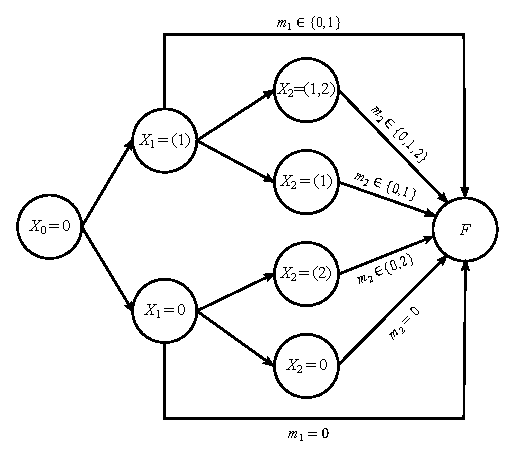
\includegraphics[scale=1]{states.eps}
\caption[]{States and transitions of the MDP for a two-channel spectrum. Arrows ending at the termination state $F$ denote transitions associated to $u_{k}=0$. The sets ${M}_{k}(x_{k})$ for these transitions are explicitly stated.}\label{fig:states}
\end{figure}

\subsection{The Equivalent MDP Problem} 
At the $k$-th stage each pair state-decision is associated to a \textit{per-stage cost}, denoted by $g_{k}\left(x_{k},d_{k}\right)$ which accumulates over time.
For the special case that $x_{k}=F$ (termination state) the per-stage cost equals $0$, therefore we can define an auxiliary function $\tilde{g}_{k}\left(x_{k},d_{k}\right)$, such that
\begin{equation}\label{generalcost}
g_{k}\left(x_{k},d_{k}\right) =
\begin{cases}
0, & \mbox{if} \quad x_{k} = F\\
\tilde{g}_{k}\left(x_{k},d_{k}\right), & \mbox{if} \quad x_{k} \in \mathcal{X}_{k}\\
\end{cases}
\end{equation}
Because the termination state is absorbing, no additional cost is accumulated when the CP system reaches it.
%Moreover, since the scanning decision at stage $N$ is always $u_{N}=0$ the cost
In our context, $\tilde{g}_{k}\left(x_{k},d_{k}\right)$ may estimate the overlapping time, the throughput or a combination of both. 
The formulation of the objectives and therefore the computation of the per-stage cost is addressed in Section \ref{sec:Policies}.

The objective of the finite-horizon MDP is to find a policy $\eta=\left\{\mu_{0},\mu_{1},\ldots,\mu_{N}\right\}$ that minimizes the \textit{cost function}
\begin{equation}\label{totalCost}
J_{\eta} = \underset{X^{*}_0,\ldots,X^{*}_N}{\mathbb{E}}\left\{\displaystyle\sum_{k=0}^{N}g_{k}\left(X^{*}_{k},\mu_{k}\left(X^{*}_{k}\right)\right)\right\}
%J_{\eta} = \underset{\vec{X}_{k}}{E}
%\left\{\displaystyle\sum_{k=0}^{N}g_{k}\left(\vec{X}_{k},\mu_{k}\left(\vec{X}_{k}\right)\right)\right\}
\end{equation}
In compact notation the MDP problem consists of finding the optimal cost $J^{*}$
\begin{equation}\label{MDPproblem}
J^{*} = \underset{\eta}{\mbox{min }} J_{\eta}
\end{equation}

%probabilidades de transici�n.
The computation of the expectation on the right hand side of (\ref{totalCost}) relies on the transition probabilities $p_{k}\left(x_{k+1} | x_{k}, d_{k}\right)$, providing the probability of making a transition from state $x_{k}$ in time $k$ to state $x_{k+1}$ in time $k+1$ when the decision is $d_{k}=\left(u_{k},\cdot\right)$.\footnote{Note that $m_{k}$ does not affect the transition probabilities of $x_{k}$.}
%Let us see how to compute these probabilities.
%The finite-horizon MDP consist of finding the optimal cost $J^{*}$
%\begin{equation}\label{totalCost}
%J^{*} = \underset{\begin{subarray}{c} \mu_{k}\\k=0,\ldots,N\end{subarray}}{\mbox{min}}
%\displaystyle\sum_{k=0}^{N}\displaystyle\sum_{j\in \mathcal{X}_{k+1}^{*}}
%p_{k}\left(j| x_{k}, u_{k}\right)
%g_{k}\left(x_{k},\mu_{k}\left(x_{k}\right)\right)
%\end{equation}

%Therefore, we have to characterize the transition probabilities for $\vec{X}_{k}$. 

\subsection{Computing the Transition Probabilities}
The transition probabilities $p_{k}\left(x_{k+1} | x_{k}, u_{k}\right)$  for every $x_{k},x_{k+1}\in \mathcal{X}_{k}$, $u_{k}\in \mathcal{U}_{k}$, $k$ = $0,\ldots,N-1$, are:
\begin{equation}
p_{k}\left(x_{k+1} | x_{k}, u_{k}\right) =
\begin{cases}
%\begin{array}{l}
1, \quad \mbox{if} \quad x_{k} = F \mbox{ and } x_{k+1} = F\\
0, \quad \mbox{if} \quad x_{k} = F \mbox{ and } x_{k+1} \neq F\\
(1-u_{k}), \quad \mbox{if} \quad x_{k} \neq F, x_{k+1} = F\\
u_{k}P\left(X_{k+1}=x_{k+1}|x_{k}\right), \mbox{otherwise}\\
%\end{array}
\end{cases}
\end{equation}
where $P\left(X_{k+1}=x_{k+1}|x_{k}\right)$ denotes the probability that the information vector equals $x_{k+1}$ at stage $k+1$ conditioned on its value $x_{k}$ at previous stage.
Let us describe how to compute $P\left(X_{k+1}=x_{k+1}|x_{k}\right)$.
%$\vec{X}_{k} = x_{k}$, for $x_{k+1}  \in \mathcal{X}_{k+1}$ and $x_{k} \in \mathcal{X}_{k}$.

Recall that each state $x_{k}$ depends on the observed process $Y_{k}$. 
At the initial state $x_{0}$, where no observation is still available, $Y_{0}$ is a random variable, characterized by a probability distribution that we will denote by $\vec{\pi}_{0}$. Because the spectrum process $Y(t)$ is active long before secondary users attempt to access the spectrum, the probability distribution $\vec{\pi}_{0}$ can be assumed to be the steady-state probability distribution (\textit{probability vector}) of $Y_{k}$. The transition probability matrix of $Y_{k}$, $\mat{P}(t)$, is obtained from the Kolmogorov \textit{forward} equation
\begin{equation}\label{Kolmogorov}
\displaystyle\frac{d\mat{P}\left(t\right)}{dt}=\mat{P}(t)\mat{Q}
\end{equation}
The elements $p_{ij}(t)$ of $\mat{P}(t)$ provide the transition probabilities between any pair of states, $i$, $j$ $\in \mathcal{S}$ of $Y(t)$ when the process runs for $t$ units of time. Since $Y_{k}$ = $Y\left(k\tau\right)$, the transition matrix for $Y_{k}$ is $\mat{P} = \mat{P}(\tau)$. The solution of (\ref{Kolmogorov}) is $\mat{P}(t)=e^{t\mat{Q}}$, therefore:
\begin{equation}\label{TransitionMatrix}
\mat{P} = \mat{P}(\tau)=e^{\tau \mat{Q}}
\end{equation}
The probability vector $\vec{\pi}_{0}$ is the unique solution to the equations below:
\begin{equation}\label{linearEquation}
\vec{\pi}_{0} = \vec{\pi}_{0}\mat{P}, \quad \left\|\vec{\pi}_{0}\right\|_{1}=1
\end{equation} 

Let us define two additional probability distributions, $\vec{\pi}_{x_{k}}$, and $\hat{\vec{\pi}}_{x_{k}}$, required to obtain $P\left(X_{k+1}=x_{k+1}|x_{k}\right)$.  
First, let $\vec{\pi}_{x_{k}}$ denote the probability distribution of $Y_{k}$ given the information vector $x_{k}$:
\begin{equation}
\vec{\pi}_{x_{k}}(i) = P\left(Y_{k}=i | x_{k}\right), \quad \text{for } i \in \mathcal{S}
\end{equation}
Second, let $\hat{\vec{\pi}}_{x_{k}}$ denote the probability distribution of $Y_{k+1}$ estimated when the available information is $x_{k}$:
\begin{equation}
\hat{\vec{\pi}}_{x_{k}}(i) = P\left(Y_{k+1}=i | x_{k}\right), \quad \text{for } i \in \mathcal{S}
\end{equation}
Essentially, $\hat{\vec{\pi}}_{x_{k}}$ is an \textit{a priori} estimate of the distribution of $Y_{k+1}$, \textit{i.e.} before receiving the observation $z_{k+1}$ at stage $k+1$.
Once $z_{k+1}$ is known, it is possible to compute the \textit{a posteriori} estimate of $Y_{k+1}$, $\vec{\pi}_{x_{k+1}}$. 

For the perfect detection case, the conditional probability $P\left(X_{k+1}=x_{k+1}|x_{k}\right)$ is related to $\hat{\vec{\pi}}_{x_{k}}$ by the following equation:
\begin{equation}\label{conditional}
\begin{array}{lcl}
P\left(X_{k+1}=x_{k+1}|x_{k}\right) & = & P\left(Z_{k+1}=z_{k+1}|x_{k}\right)\\
 & = & P\left(Y_{k+1} \in \mathcal{S}(k+1,z_{k+1})|x_{k}\right)\\
& = & \displaystyle\sum_{j \in \mathcal{S}(k+1,z_{k+1})}P\left(Y_{k+1} = j|x_{k}\right)\\
& = & \displaystyle\sum_{j \in \mathcal{S}(k+1,z_{k+1})}\hat{\vec{\pi}}_{x_{k}}(j)
\end{array}
\end{equation}

For the imperfect detection case, the conditional probability $P\left(\vec{X}_{k}=x_{k}|x_{k-1}\right)$ is given by
\begin{equation}\label{conditionalcomplete}
\begin{array}{lcl}
P\left(\vec{X}_{k}=x_{k}|x_{k-1}\right) & = & P\left(Z_{k}=z_{k}|x_{k-1}\right)\\
 & = & P\left(Y_{k} \in \mathcal{S}(k,z_{k})|x_{k-1}\right)p_{c}(z_{k}) + \\
 && P\left(Y_{k} \in \mathcal{S}^{c}(k,z_{k})|x_{k-1}\right)p_{i}(z_{k}) \\
 & = & \displaystyle\sum_{j \in \mathcal{S}(k,z_{k})}P\left(Y_{k} = j|x_{k-1}\right)p_{c}(z_{k}) +\\
 && \displaystyle\sum_{j \in \mathcal{S}^{c}(k,z_{k})}P\left(Y_{k} = j|x_{k-1}\right)p_{i}(z_{k}) \\
 & = & \displaystyle\sum_{j \in \mathcal{S}(k,z_{k})}\hat{\vec{\pi}}_{x_{k-1}}(j)p_{c}(z_{k}) + \\
 && \displaystyle\sum_{j \in \mathcal{S}^{c}(k,z_{k})}\hat{\vec{\pi}}_{x_{k-1}}(j)p_{i}(z_{k})
\end{array}
\end{equation}

Now we specify how to compute the conditional distributions $\hat{\vec{\pi}}_{x_{k}}$ and $\vec{\pi}_{x_{k}}$.
The conditional distribution $\hat{\vec{\pi}}_{x_{k}}$ can be obtained from the \textit{a posteriori} estimate of previous stage $\vec{\pi}_{x_{k-1}}$  
\begin{equation}
\begin{array}{lcl}
\hat{\vec{\pi}}_{x_{k}}(i) & = & P\left(Y_{k+1}=i | x_{k}\right) \\
										& = & \sum_{j\in \mathcal{S}}P\left(Y_{k+1}=i | Y_{k}=j\right)P\left(Y_{k}=j | x_{k-1}\right)\\
										& = & \sum_{j\in \mathcal{S}}p_{ji}\vec{\pi}_{x_{k-1}}(j)
\end{array}
\end{equation}
for $i\in \mathcal{S}$, where $p_{ji}$ are the elements of the transition matrix $P$ obtained in (\ref{TransitionMatrix}). Using vector notation we have $\hat{\vec{\pi}}_{x_{k}} = \vec{\pi}_{x_{k}}P$.

Regarding $\vec{\pi}_{x_{k}}$, for the particular case of $x_{0}$ we have, by definition
\begin{equation}
\vec{\pi}_{x_{0}}(i) = P\left(Y_{0}=i\right) = \vec{\pi}_{0}(i), \quad \text{for } i \in \mathcal{S}
\end{equation}
and, for $k=1,\ldots,N$ we have, for the perfect detection case: 
\begin{equation}
\begin{array}{lcl}
\vec{\pi}_{x_{k}}(i) &=& P\left(Y_{k}=i | x_{k}\right)\\
					 &=& P\left(Y_{k}=i | z_{k}, x_{k-1}\right)\\
					 &=& \displaystyle\frac{P\left(Y_{k}=i, Z_{k}=z_{k} | x_{k-1}\right)}{P\left(Z_{k}=z_{k} | x_{k-1}\right)}\\
					 &=& 
\begin{cases}
\displaystyle\frac{P\left(Y_{k}=i | x_{k-1}\right)}{P\left(Z_{k}=z_{k} | x_{k-1}\right)},& \mbox{if} \quad i \in \mathcal{S}(k,z_{k})\\
0, & \mbox{otherwise}\\
\end{cases}\\
\end{array}
\end{equation}
where $P\left(Y_{k}=i | x_{k-1}\right) = \hat{\vec{\pi}}_{x_{k-1}}(i)$, and $P\left(Z_{k}=z_{k} | x_{k-1}\right)$ is given by (\ref{conditional}). And for the imperfect detection case: 
\begin{equation}
\begin{array}{lcl}
\vec{\pi}_{x_{k}}(i) &=& P\left(Y_{k}=i | x_{k}\right)\\
					 &=& P\left(Y_{k}=i | z_{k}, x_{k-1}\right)\\
					 &=& \displaystyle\frac{P\left(Y_{k}=i, Z_{k}=z_{k} | x_{k-1}\right)}{P\left(Z_{k}=z_{k} | x_{k-1}\right)}\\
					 &=& 
\begin{cases}
\displaystyle\frac{P\left(Y_{k}=i | x_{k-1}\right)p_{c}(z_{k})}{P\left(Z_{k}=z_{k} | x_{k-1}\right)},& \mbox{if} \quad i \in \mathcal{S}(k,z_{k})\\
\displaystyle\frac{P\left(Y_{k}=i | x_{k-1}\right)p_{i}(z_{k})}{P\left(Z_{k}=z_{k} | x_{k-1}\right)},& \mbox{if} \quad i \in \mathcal{S}^{c}(k,z_{k})\\
\end{cases}\\
\end{array}
\end{equation}
where $P\left(Y_{k}=i | x_{k-1}\right) = \hat{\vec{\pi}}_{x_{k-1}}(i)$, and $P\left(Z_{k}=z_{k} | x_{k-1}\right)$ is given by (\ref{conditionalcomplete}).
Summarizing, the conditional distributions $\hat{\vec{\pi}}_{x_{k}}$ and $\vec{\pi}_{x_{k}}$ can be recursively generated starting with
\begin{equation}
\vec{\pi}_{x_{0}} = \vec{\pi}_{0},
\end{equation}
and using the following equations. For the perfect detection case: 
\begin{equation}\label{recursive}
\begin{array}{lcl}
\hat{\vec{\pi}}_{x_{k-1}} & = & \vec{\pi}_{x_{k-1}}\mat{P},\\
\vec{\pi}_{x_{k}}(i) &=& 
\begin{cases}
\displaystyle\frac{\hat{\vec{\pi}}_{x_{k-1}}(i)}{\sum_{j \in \mathcal{S}(k,z_{k})}\hat{\vec{\pi}}_{x_{k-1}}(j)},& \mbox{if} \quad i \in \mathcal{S}(k,z_{k})\\
0, & \mbox{otherwise}\\
\end{cases}\\
\end{array}
\end{equation}
for $k = 1,\ldots,N$. And for the imperfect detection case: 
\begin{equation}\label{recursive2}
\begin{array}{lcl}
\hat{\vec{\pi}}_{x_{k-1}} & = & \vec{\pi}_{x_{k-1}}\mat{P},\\ 
\vec{\pi}_{x_{k}}(i) & = & 
\begin{cases}
\displaystyle\frac{\hat{\vec{\pi}}_{x_{k-1}}(i)p_{c}(z_{k})}{\displaystyle
{\sum_{\mathrlap{j \in \mathcal{S}(k,z_{k})}}}\hat{\vec{\pi}}_{x_{k-1}}(j)p_{c}(z_{k}) + \displaystyle{\sum_{\mathclap{j \in \mathcal{S}^{c}(k,z_{k})}}}\hat{\vec{\pi}}_{x_{k-1}}(j)p_{i}(z_{k})},& \mbox{if} \quad i \in \mathcal{S}(k,z_{k})\\
\displaystyle\frac{\hat{\vec{\pi}}_{x_{k-1}}(i)p_{i}(z_{k})}{\displaystyle{\sum_{\mathrlap{j \in \mathcal{S}(k,z_{k})}}}\hat{\vec{\pi}}_{x_{k-1}}(j)p_{c}(z_{k}) + \displaystyle{\sum_{\mathclap{j \in \mathcal{S}^{c}(k,z_{k})}}}\hat{\vec{\pi}}_{x_{k-1}}(j)p_{i}(z_{k})},& \mbox{if} \quad i \in \mathcal{S}^{c}(k,z_{k})\\
\end{cases}\\
\end{array}
\end{equation}
for $k = 1,\ldots,N$.

\section{Obtaining Pareto-Optimal Policies}\label{sec:Policies}
\subsection{Cost Function}
%In cognitive radio access there is, in general, a trade-off between secondary user transmission rate (\textit{throughput}) and collision probability with licensed users. 
The cost function $\tilde{g}_{k}(x_{k},d_{k})$ represents a convex combination of two opposite objectives:  the throughput $b_{k}(m_{k})$ and the average overlapping time $c_{k}(x_{k},m_{k})$:
\begin{equation}\label{cost}
\tilde{g}_{k}(x_{k},d_{k}) = \left[\alpha \frac{c_{k}(x_{k},m_{k})}{c_{\text{max}}} + (\alpha -1)\frac{b_{k}(m_{k})}{b_{\text{max}}}\right](1-u_{k})
\end{equation}
where $0\leq \alpha \leq 1$. The objectives are divided by their maximum values $c_{\text{max}}$ and $b_{\text{max}}$ in order to obtain dimensionless (normalized) values. Note that $b_{k}(x_{k},m_{k})$ is added with negative sign in the convex combination because the cost function is minimized in problem (\ref{MDPproblem}). According to multi-objective optimization theory, given a value of $\alpha$, the solution of the finite-horizon MDP with the cost defined in (\ref{cost}) yields a Pareto-optimal solution regarding these two opposite objectives, \textit{i.e.} a solution for which there does not exists any policy such that one objective can be improved without worsening the other. The set of Pareto-optimal solutions is referred to as the Pareto-front of the problem and we can estimate it by iteratively solving the MDP for a representative discrete range of $\alpha$ values.
\subsubsection{Throughput}
The maximum throughput is attained when $M$ channels are found idle in the first $M$ scanning slots and the decision made is to transmit using these $M$ channels. Given a transmission rate $R$ and scanning and transmission times equal to $\tau$ and $T$ respectively, the maximum throughput is
\begin{equation}
b_{\text{max}} = \frac{MRT}{M\tau + T}.
\end{equation}
When the access algorithm decides to transmit in $n$ channels at stage $k$ the throughput is
\begin{equation}
b_{k}(m_{k}) = \frac{nRT}{k\tau + T},\text{ } n \leq k
\end{equation}
\subsubsection{Average Overlapping Time}
The maximum average overlapping time occurs when, after selecting $M$ channels to transmit in, these $M$ channels turn out to be occupied by PUs when the SU starts to transmit and remain occupied for at least $T$ seconds. Therefore, in the worst case of having $M$ collisions lasting for $T$ seconds, the total overlapping time is:
\begin{equation}
c_{\text{max}} = MT.
\end{equation}
Accordingly, given a vector $m_{k}$ selecting $n$ channels to transmit in after the $k$-th scanning slot, the average overlapping time is given by
\begin{equation}\label{collision}
c_{k}(x_{k},m_{k}) = \displaystyle\sum_{j=1}^{n}\underset{\begin{subarray}{c} Y(t)\\t\in[k\tau, k\tau + T)\end{subarray}}{E}\Bigl[t \text{ in }\mathcal{S}(m_{k}(j),1)\Big|x_{k}\Bigr]
%c_{k}(x_{k},m_{k}) = \displaystyle\sum_{j=1}^{n}\underset{\underset{t\in[k\tau, k\tau + T)}{Y(t)}}{E}\Bigl[t \text{ in }\mathcal{S}(m_{k}(j),1)\Big|x_{k}\Bigr]
%c_{k}(x_{k},m_{k}) = \displaystyle\sum_{j=1}^{n}\underset{\begin{array}{c}_{t\in[k\tau, k\tau + T)}\\_{Y(t)}\end{array}}{\text{\large E}}\Bigl[t \text{ in }\mathcal{S}(m_{k}(j),1)\Big|x_{k}\Bigr]
\end{equation}
where the expectation operation calculates the expected total time that the spectrum process $Y(t)$ spends in the set of states $\mathcal{S}(m_{k}(j),1)$ during the period $[k\tau, k\tau + T)$. 
Recall that, according to its definition in (\ref{setS}), $\mathcal{S}(m_{k}(j),1)$ corresponds to the set of states in $\mathcal{S}$, such that channel $m_{k}(j)$ is occupied by a PU. 
Therefore, (\ref{collision}) is the sum of the expected overlapping times on each of the $n$ channels selected. Let us denote by $l_{i,x_k}(t')$ the expected total time that $Y(t)$ spends in state $i \in \mathcal{S}$ during the interval $[k\tau, k\tau+t']$ given the information $x_k$, after $k$ scanning slot. Then, 
\begin{equation}
c_{k}(x_{k},m_{k}) = \displaystyle\sum_{j=1}^{n}\displaystyle\sum_{i\in\mathcal{S}(m_{k}(j),1)}l_{i,x_{k}}(T-k\tau)
\end{equation}
The expected total time spent in a state, $l_{i,x_k}(t')$, is a known performance parameter of Markov models (see \cite{ref:Bolch2006}). Let $\vec{L}_{x_k}(t')$ indicate the vector whose elements are $l_{i,x_k}(t')$, and let $\vec{\pi}^{(t)}_{x_k}$ denote the transient state probability vector of $Y(t)$ conditioned on $x_k$.
By definition, $\vec{L}_{x_k}(t')$ can be expressed as:
\begin{equation}\label{integral}
\vec{L}_{x_k}(t') = \int_{k\tau}^{k\tau+t'}\vec{\pi}^{(t)}_{x_k} dt,
\end{equation}
At time $k\tau$, the value of $Y(t)$ is given by $Y(k\tau) = Y_{k}$, whose probability distribution conditioned on $x_{k}$ is $\vec{\pi}_{x_{k}}$. Therefore, $\vec{\pi}^{(k\tau)}_{x_k} = \vec{\pi}_{x_{k}}$, given by (\ref{recursive}) and (\ref{recursive2}), allowing us to compute $\vec{L}_{x_k}(t')$ as the solution of the following differential equation
\begin{equation}\label{equation}
\frac{d\vec{L}_{x_k}(t')}{dt'} = \vec{L}_{x_k}(t')\mat{Q} + \vec{\pi}_{x_{k}}, \quad \vec{L}_{x_k}(0)=\vec{0} 
\end{equation}
%\begin{equation}\label{timeL}
%\frac{d\vec{L}_{x_k}(\Delta t)}{d\Delta t} = \vec{L}_{x_k}(\Delta t)\mat{Q} + \vec{\pi}_{x_{k}}, \quad l_{i,x_k}(0)=0 \quad \forall i\in\mathcal{S} 
%\end{equation}
\subsection{Backward Induction Algorithm}
%Comentarios sobre las pol�ticas (HD,RD...), existencia de pol�ticas etc. Backward induction algorithm. Estimar el coste computacional.
Once the POMDP has been reformulated as a fully observable state estimation one, and given that the horizon is finite, the MDP problem can be solved by means of the backward induction algorithm, also known as dynamic programming (DP) algorithm.
In addition, because both the state and the control spaces are finite, there exists at least one deterministic Markovian policy which is optimal \cite{ref:Puterman2005}.
This is the type of policies defined in Subsection \ref{Policies}, where each function $\mu_{k}$ maps states (not past histories) into decisions, \textit{i.e.} $\mu_{k}$ is Markovian. Similarly, $\mu_{k}(x_{k})$ always gives the same outcome with probability 1, \textit{i.e.} $\mu_{k}$ is deterministic.

The algorithm to find optimal Markovian deterministic policies for the MDP problem (\ref{MDPproblem}) is the following:

\noindent\textbf{1. }Set $k=N$ and
	\begin{equation}
	J^{*}_{N}\left(x_{N}\right) = \underset{d\in\mathcal{D}_{N}(x_{N})}
	{\mbox{min }}g_{N}\left(x_{N},d\right) \mbox{ for all } x_{N} \in \mathcal{X}^{*}_{N}
	\end{equation}
	Set
	\begin{equation}\label{muNpolicy}
	\mu^{*}_{N}(x_{N}) = \underset{d\in\mathcal{D}_{N}(x_{N})}
	{\mbox{arg max }}g_{N}\left(x_{N},d\right).
	\end{equation}
\textbf{2. }Substitute $k-1$ for $k$ and compute $J^{*}_{k}\left(x_{k}\right)$ for each $x_{k}~\in~\mathcal{X}^{*}_{k}$ by
\begin{equation}\label{Jkcost}
J^{*}_{k}\left(x_{k}\right) = \underset{d\in\mathcal{D}_{k}(x_{k})}
{\mbox{min }}\left\{g_{k}\left(x_{k},d\right) + \displaystyle\sum_{j\in\mathcal{X}^{*}_{k}}p_{k}\left(j|x_{k},d\right)J^{*}_{k+1}\left(j\right)\right\}
\end{equation}
Set
\begin{equation}\label{mukpolicy}
\hspace{3em}\mu^{*}_{k}(x_{k}) = \underset{d\in\mathcal{D}_{k}(x_{k})}
{\mbox{arg min }}\left\{g_{k}\left(x_{k},d\right) + \displaystyle\sum_{j\in\mathcal{X}^{*}_{k}}p_{k}\left(j|x_{k},d\right)J^{*}_{k+1}\left(j\right)\right\}
\end{equation}
\textbf{3. }If $k=0$ stop. Otherwise return to step 2.

At the end of previous algorithm, (\ref{Jkcost}) provides the optimal cost function for $k=0$, $J^{*}_{0}\left(x_{0}\right)$. Because the scanning process starts with null initial information, \textit{ i.e.} $x_{0}=0$, the scalar value $J^{*}_{0}\left(0\right)$ is the optimal cost $J^{*}$ defined in (\ref{MDPproblem}).
Note that both (\ref{muNpolicy}) and (\ref{mukpolicy}) may result in more than one optimal decision per state, meaning that there may be more than one optimal policy $\eta^{*}$ for the problem.

%%Computational cost
\subsection{Computational Cost}
%This subsection is concerned with the computational cost of obtaining an optimal OSA policy.
Given the dimension of the problem $N$, and the spectrum management policy, it is straightforward to evaluate the computational cost of obtaining the optimal OSA policy.
Table \ref{Table2} shows the computational costs, including computation time in a 50 Gflops processor, for the case of random or sequential channel allocations, considering different number of channels $N$. % The worst case implies storing $2^{N}$ decisions. Table \ref{Table2} table also shows the memory requirements to store the OSA policy.
Even if the policy is computed off-line, the computational effort becomes cumbersome for a spectrum size of around 20 channels. Nevertheless, a pre-computed policy implies memory requirements too. Considering the decision tree structure of the MDP (see Fig. \ref{fig:states}) an SU only needs to store the information states where a transmission decision has to be made. Table \ref{Table2} shows the worst case, in which $2^{N}$ states should are stored. %The SU's storage requirement results impractical around this value too.

Therefore, for larger $N$ values, approximation methods could be applied. For example, an approximate evaluation of matrix $P$, or state aggregation \textit{e.g.} by modeling PU channel occupation in blocks of channels instead of individual ones. %This issue lies beyond the scope of this work.
On the other hand, with the merged spectrum strategy, the implementation requirements of OSA reduce dramatically as shown in Table \ref{Table3}. This advantage adds to the ones shown in following section.

\begin{table}
\begin{tabular}{cccc} \hline
\textbf{channels} & \textbf{memory} (bytes) & \textbf{multiplications} & \textbf{time} (hours)\\\hline
4 & 16 & 85296 & $4.7\times10^{-10}$\\
8 & 256 & $3.1\times10^{8}$ & $1.7\times10^{-6}$\\
12 & 4096 & $1.3\times10^{12}$ & 0.007\\
16 & 65536 & $5.2\times10^{15}$ & 28.67\\
20 & 1048576 & $2.1\times10^{19}$ & 117427\\
24 & $1.7\times10^{7}$ & $8.7\times10^{22}$ & $4.8\times10^{8}$\\\hline
\end{tabular}
\centering
\caption{Off-line computational effort and SU memory requirements for OSA under random or sequential PU channel assignment}
\label{Table2}
\end{table}

\begin{table}
\begin{tabular}{cccc} \hline
\textbf{channels} & \textbf{memory} (bytes) & \textbf{multiplications} & \textbf{time} (seconds)\\\hline
4 & 4 & 1804 & $3.6\times10^{-8}$\\
8 & 8 & 11928 & $2.4\times10^{-7}$\\
12 & 12 & 37412 & $7.5\times10^{-7}$\\
16 & 16 & 85296 & $1.7\times10^{-6}$\\
20 & 20 & 162620 & $3.3\times10^{-6}$\\
24 & 24 & 276424 & $5.5\times10^{-6}$\\\hline
\end{tabular}
\centering
\caption{Off-line computational effort and SU memory requirements for OSA under spectrum merging for PUs}
\label{Table3}
\end{table}

\section{Numerical Results}\label{ref:Results}
\subsection{Performance Evaluation}
In this subsection we compare the performance of Pareto-optimal OSA policies for the three PU channel allocation strategies previously explained: random, sequential and sequential with spectrum merging for PUs. We use a Poisson traffic model, with 8 new PU arrivals per minute, and and average channel holding time of 1 minute, i.e. an offered traffic of 8 Erlangs over a 10-channels band.
The parameter settings of the evaluation scenario are shown in Table \ref{Table4}.

\begin{table}[ht]
\begin{tabular}{lr} \hline
\textbf{Parameter} & \textbf{Value} \\\hline
$N$ & $10$ channels\\
$M$ & $3$ channels\\
$\lambda$ & $\frac{8}{60}\text{ }s^{-1}$\\
$1/\mu$ & $60\text{ }s$\\
$T$ & $10\text{ }s$\\
$\tau$ & $500\text{ }ms$\\\hline
\end{tabular}
\centering
\caption{Parameter settings}
\label{Table4}
\end{table}

As explained in previous section, the per-stage cost function (\ref{cost}) consists of a convex combination of two opposite parameters: throughput and overlapping time. For a given weight $\alpha$ in (\ref{cost}), a policy $\eta^{*}$ solving the MDP problem yields an expected normalized throughput, denoted by $J_{\text{th}}$ and an expected total overlapping time denoted by $J_{c}$. %The policy $\eta^{*}$ is Pareto-optimal because $J_{\text{th}}$ cannot be improved by any other policy without worsening $J_{c}$ and \textit{vice versa}.
For any policy $\eta = \left\{\mu_{0},\ldots,\mu_{N}\right\}$, $J_{\text{th}}$ is obtained by the following recursive equations:
\begin{equation}
	J_{\text{th},k}\left(x_{k}\right) = g_{\text{th},k}\left(x_{k},\mu_{k}\left(x_{k}\right)\right) + \displaystyle\sum_{j\in\mathcal{X}^{*}_{k}}
	p_{k}\left(j|x_{k},\mu_{k}\left(x_{k}\right)\right)J_{\text{th},k+1}\left(j\right)
\end{equation}
for $k=N-1,\ldots,0$, starting with
\begin{equation}
	J_{\text{th},N}\left(x_{N}\right) = g_{\text{th},N}\left(x_{N},\mu_{N}\left(x_{N}\right)\right) \mbox{ for all } x_{N} \in \mathcal{X}^{*}_{N}.
\end{equation}
In these equations, $g_{\text{th},k}$ denotes the per stage throughput and is given by (\ref{generalcost}) and (\ref{cost}) with $\alpha = 1$. The total throughput is $J_{\text{th}} = J_{\text{th},0}\left(x_{0}\right)$. The expected total overlapping time $J_{c}$ is obtained similarly.


Fig. \ref{fig:paretofront} shows the Pareto fronts obtained under the three PU channel allocation patterns considered. As expected, OSA performs better when channels are assigned sequentially to PUs, and much better when PUs always occupy adjacent channels into a compacted spectrum block. To give an idea of this improvement, let us set the constraint $J_{c}\leq0.1$. Depending on how PU channels are managed, the maximum achievable $J_{\text{th}}$ can be 0.4, 0.58 or 0.7. Conversely, if the goal is to keep $J_{\text{th}}$ close to 0.6, the minimum achievable $J_{c}$ values are 0.35, 0.14 or 0.03 for each PU channel management strategy. 
%Conversely, if the objective is to achieve a normalized SU throughput equal to 0.6, the minimum achievable collision time can be 0.35, 0.14 or 0.03.

\begin{figure}[ht]
\centering
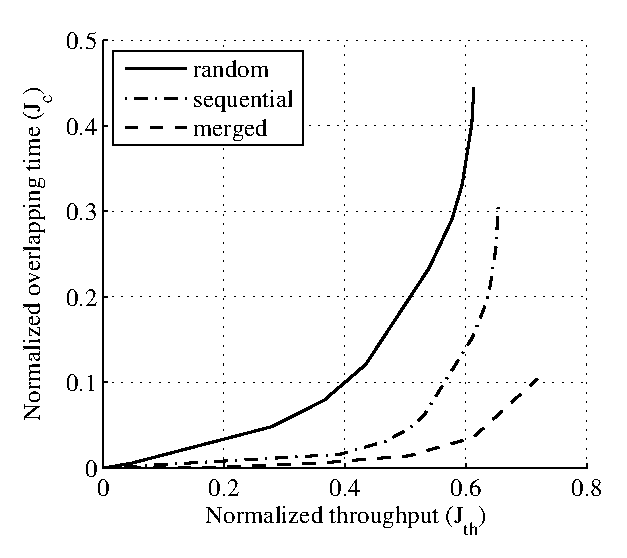
\includegraphics[scale=0.7]{ParetoFront10.eps}
\caption[]{Pareto fronts showing the optimal combinations of normalized optimal throughput and normalized overlapping time for three different PU channel allocation patterns.}\label{fig:paretofront}
\end{figure}

To show the benefit of MDP-based policies let us consider the following family of \textit{baseline policies}, $\eta^{r}$: A CP following $\eta^{r}$ decides to transmit over $M$ channels whenever the number of available channels detected is $n_{f} = M + r$. Otherwise, the CP pair keeps on scanning the spectrum. If the total number of available channels in the spectrum is $n_{f} < M + r$, then the SU node transmits in $n=\text{max}\left(n_{f}-r,0\right)$ channels.
%\begin{equation}
%n = 
%	\begin{cases}
%	n_{f}-r &, \mbox{if} \quad n_{f} > r\\
%	0 &, \mbox{otherwise}\\
%	\end{cases}	
%\end{equation}
The integer parameter $r > 0$ represents a bandwidth safety margin to reduce collisions. Fig. \ref{fig:comparative} compares the performance of baseline policies $\eta^{r}$ for $r = 0,\ldots,N-1$, to MDP-based policies under each PU channel management scheme. Note that the lower the safety margin $r$, the greater the throughput, at the cost of an increased overlapping time. Although MDP-based policies outperform the reference ones in every scenario, it is interesting how close the reference performance is to the Pareto front in the merged spectrum scenario, suggesting that, in this case, it may be acceptable to use a simple set of rules similar to $\eta^{r}$, alleviating the need to solve the MDP problem off-line.
This also illustrates the utility of Pareto front computations for evaluating OSA policies. The performance of both sets of policies is also similar under every PU strategy for the case in which the overlapping time is of no importance ($\alpha = 0$), since both decide to transmit over the maximum $M$ channels (if $M$ or more channels are available). 
%suggesting that the Pareto-optimal policies in this case can be reduced to a simple set of rules similar to $\eta^{r}$. 

\begin{figure}[ht]
\centering
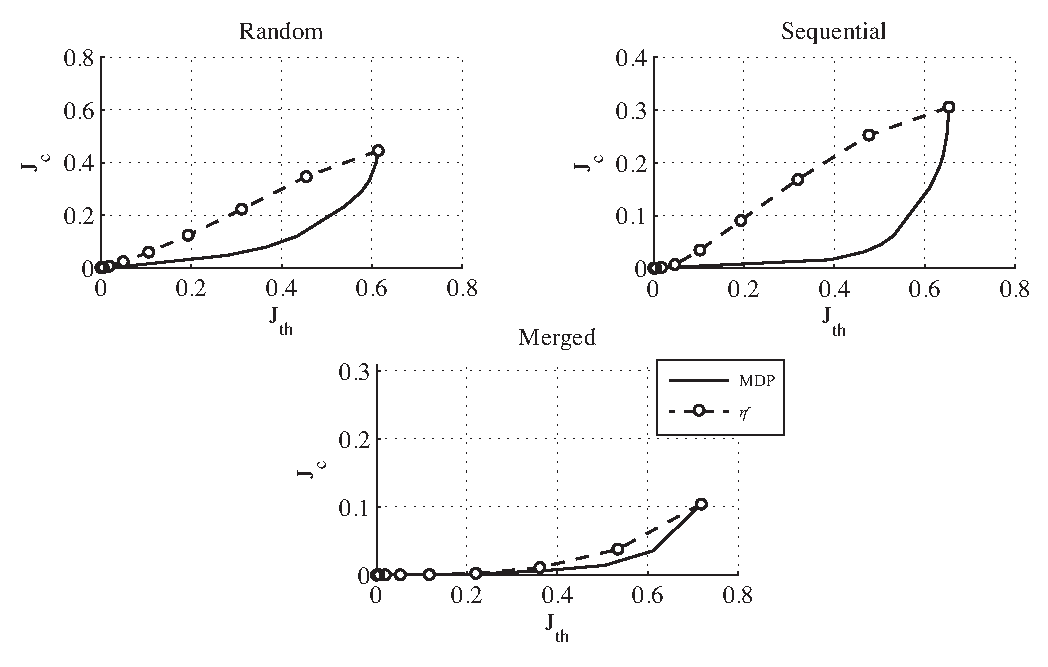
\includegraphics[scale=0.8]{ReferencePolicies.eps}
\caption[]{MDP-based policies \textit{vs.} baseline policies $\eta^{r}$ with $r = 0,\ldots,N-1$.}\label{fig:comparative}
\end{figure}

One reasonable concern about the proposed procedure for obtaining OSA policies is that it may be too reliant on PU traffic estimation accuracy. 
Even if the Poisson model is suitable for PU traffic, the $\lambda$ and $\mu$ values used for off-line policy computation may be very different from realistic ones, which may also change over time.
The question is how much does the accuracy of traffic descriptors affect the performance figures, especially overlapping time which determines the QoS of PUs.
%Even if Poisson model is suitable for PU traffic, real $\lambda$ and $\mu$ values may be very different from the values used in the off-line policy computation and they may change over time.
Next subsection addresses this issue. 
%therefore the throughput obtained with this policy cannot be improved without worsening the collision time. 

\subsection{Sensitivity to Traffic Estimation Accuracy}
This subsection evaluates the sensitivity of each performance figure to drifts on the values of PU traffic descriptors $\lambda$ and $\mu$. By drift we refer to the difference between the value used for off-line policy computation (estimated value) and the value that actually describes PU traffic (nominal value). 
Drifts are positive when PU traffic is larger than the estimated one, and negative otherwise.

%To perform this evaluation we selected, for each PU channel assignment scheme, a Pareto-optimal policy computed using the $\lambda$ and $\mu$ values specified in Table \ref{Table4}.
For the three PU channel management scenarios considered so far, the OSA policy is computed using the nominal $\lambda$ and $\mu$ values specified in Table \ref{Table4}.
Then, at each scenario, we evaluated the performance of the OSA policy in terms of throughput and overlapping time for drifts ranging from negative to positive values.
In OSA, the main concern is to keep PU's QoS degradation at low values.
%CONSIDERAR: explicar como se ha computado cada par�metro (recursivamente, etc).
Therefore, selected OSA policies have low overlapping times at nominal traffic descriptors, as shown in Table \ref{Table5}. 
%Note that these measures correspond to the reference scenario with zero drift.

%Because in OSA the main concern is to assure PU QoS, the policies selected attain low collision times. Table \ref{Table5} shows the performance measures for each PU channel allocation pattern in the reference scenario with zero drift.
%Because in OSA the main concern is to assure PU QoS, we have selected Pareto-optimal policies with low collision times. Table \ref{Table5} shows the performance measures for each PU channel allocation pattern in the reference scenario with zero drift.
%The larger the difference, the less accurate the traffic estimation is.

\begin{table}[ht]
\begin{tabular}{lccc} \hline
\textbf{PU channel allocation} & random & sequential & merged\\\hline
\textbf{normalized throughput} & 0.43 & 0.53 & 0.72\\
\textbf{normalized overlapping time}  & 0.12 & 0.06 & 0.10\\\hline
\end{tabular}
\centering
\caption{Performance figures in the reference scenario with zero drift.}
\label{Table5}
\end{table}

Fig. \ref{fig:random} shows the throughput and overlapping time values attained by the OSA policy in a system with random PU channel assignment, for different combinations of the estimated $\lambda$ and $\mu$ values. 
%The reference policy is computed for $\lambda = \frac{8}{60}$ and $\mu = \frac{1}{60}$, thus the figure shows the results for negative and positive drifts on both parameters.
The nominal traffic descriptors are $\lambda = \frac{8}{60}$ s$^{-1}$ (8 arrivals per minute) and $\mu = \frac{1}{60}$ s$^{-1}$ (average holding time: 1 minute), thus the axis in Fig. \ref{fig:random} contains negative and positive drifts on both parameters.  
It was expectable that positive and negative drifts resulted in reduced and improved throughput respectively.
Nevertheless, the overlapping time remains at relatively low values for every combination of $\lambda$ and $\mu$. This shows a very desirable feature of the OSA strategy proposed: contrary to the usual belief, PU traffic estimation inaccuracies have little impact on PU's QoS. This effect is also observed in the scenarios of sequential PU channel assignment (see Fig. \ref{fig:seq}) and spectrum merging for PUs (see Fig. \ref{fig:comp}). 

Clearly, if real PU traffic is heavier than predicted, the SU sensing process will provide, more frequently, observations corresponding to congested spectrum states.
Therefore, independently of the accuracy of the traffic estimation, if the policy is intended to operate with low overlapping time, it will make the conservative decisions associated to these spectrum states.
The only difference is that these decisions will be made more frequently.
%Therefore, when traffic intensity is underestimated, conservative decisions are simply made more often than expected.
%Therefore, independently of the prediction used to compute the OSA policy, if the policy is intended to operate with low collision time, it will make the conservative decisions associated to these spectrum states.
%The consequence is that, in many cases, positive drifts result in reduced overlapping time.
The consequence is that, in many cases, the overlapping time is even reduced under positive drifts.
This is not always the case in systems with spectrum merging for PUs, which is expectable because in this scenario channels are more intensively used than in the others.

\begin{figure}[ht]
\centering
\includegraphics[scale=0.6,clip]{ThroughputRandom.eps}
\includegraphics[scale=0.6,clip]{CollisionRandom.eps}
\caption[]{Normalized SU throughput and expected overlapping time with random channel assignment for PUs ($\lambda$ is given in arrivals per minute).}\label{fig:random}
\end{figure}

\begin{figure}[ht]
\centering
\includegraphics[scale=0.6,clip]{ThroughputSeq.eps}
\includegraphics[scale=0.6,clip]{CollisionSeq.eps}
\caption[]{Normalized SU throughput and expected overlapping time with sequential channel assignment for PUs ($\lambda$ is given in arrivals per minute).}\label{fig:seq}
\end{figure}

\begin{figure}[ht]
\centering
\includegraphics[scale=0.6,clip]{ThroughputComp.eps}
\includegraphics[scale=0.6,clip]{CollisionComp.eps}
\caption[]{Normalized SU throughput and expected overlapping time with spectrum merging for PUs ($\lambda$ is given in arrivals per minute).}\label{fig:comp}
\end{figure}

\section{Conclusions}\label{SPEC_MAN_sec_conclusion}
We have addressed the design of OSA policies for hardware constrained cognitive networks, and the impact of different levels of coexistence friendliness of the PU.
 % operating in an ad-hoc distributed way 
The problem was formulated as a partially observable Markov decision process with finite horizon in which, at the end of each scanning slot, the spectrum state estimation is updated considering not only the new observation but also the effect of the delay on older observations.
OSA policies need to balance SU's throughput and performance degradation of PUs, characterized by the overlapping time, which is a more general metric than collision probability.
%At the end of each scanning slot, the estimation of the spectrum occupancy probabilities is uptated considering the new observation and the increasing duration of the sensing phase.
%Hemos abordado el problema de dise�o de pol�ticas OSA para nodos con limitaciones hardware, equilibrando SU throughput y PU performance. Para ello se ha empleado una formulaci�n partaially obs. MDP, con horizonte finito, donde se observa que con el paso de las etapas la estimaci�n del estado del canal var�a no solo con las nuevas observaciones sino tambi�n por el tiempo transcurrido desde las observaciones anteriores. Para estimar la calidad de servicio de los PU se ha optado por el overlapping time al ser m�s general que la proba de colisi�n. 
Regarding the PU allocation schemes, the overall performance improves when channels are assigned to PUs sequentially instead of randomly and improves even more if PUs always occupy adjacent channels.
%Pareto front representations  
We also showed the robustness of Pareto-optimal policies against inaccuracies in PU traffic estimation, supporting the use of off-line pre-computed policies.
%Depending on how the channels are assigned to PUs and the total amount of channels, approximate methods may be required to address the problem. %Exploring these methods is an interesting future research issue.
The results described in this chapter also reinforce the idea that, in situations of low or moderate PU traffic in which the operation of cognitive networks is justified, it is convenient for the licensed network to adjust its own channel allocation polices to facilitate spectrum sharing with SUs. 
%Similarly, it is still required a wider study of the costs and the benefits of modifying licensed spectrum management in overlay scenarios.
%However, the results presented in this paper suggest that, in situations of low or moderate PU traffic, in which the operation of cognitive networks is justified, it is convenient for the licensed network to adjust its own channel allocation polices to facilitate spectrum sharing with SUs. 